\chapter{AMQP Integration Patterns}\label{chap:amqp_patterns}



\section{AMQP and Data Delivery}
The AMQP output capability is designed to fit the needs of Enterprise users that have the need for advanced data handling.  The use of AMQP allows
for delivery of data at scale to multiple consumers.  Figure \ref{fig:AMQP-data-flows} shows an example of how an Enterprise could use the
CxAnalytix AMQP output capability.

\noindent\\The Exchange and Queue capabilities defined by the AMQP protocol can enhance Enterprise data consumption patterns.  While the use
of a persistent output such as Log4Net or MongoDB are useful for storing data, AMQP can be used to store data, transform the data for storage
as subsets of data, and perform stream analysis on the data \textit{in parallel.}  

\begin{figure}[h]
    \caption{AMQP Data Flow for Enterprise Data Consolidation}
    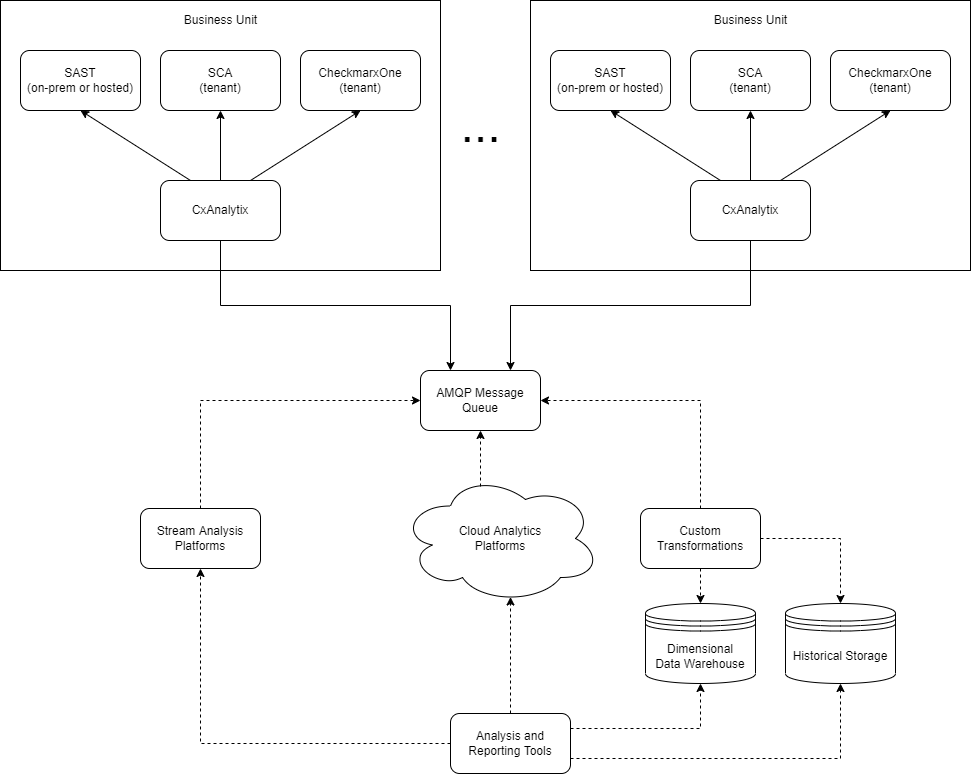
\includegraphics[width=\textwidth]{graphics/AMQP-data-org.png}
    \label{fig:AMQP-data-flows}
\end{figure}



\section{AMQP Output Messages}

\subsection{Message Generation Markers}

Every message sent by CxAnalytix contains a header with the name \texttt{Generation} having the value of \texttt{0}.  This indicates the message
has been generated as part of crawling recent scan data. The purpose of the \texttt{Generation} header is to allow the selective routing of 
"original" messages vs. messages that may be re-submitted for re-processing. 

\noindent\\As with any data analysis, the need for additional analysis may be realized as time progresses.  Storing the raw data generated by
CxAnalytix means that new analysis domains can utilize historical data as well as new data.  If the new analysis domain were to use streams
of data obtained by AMQP, all that would be required is to replay the historical CxAnalytix data.  Replay data tagged with a \texttt{Generation}
header larger than \texttt{0} could co-exist with new data submitted by CxAnalytix messages tagged as \texttt{Generation 0}.  The AMQP routing
would then route \texttt{Generation 0} messages to consumers designed to process new scan data.  This routing could be in parallel with other 
data consumers that are processing both historical data and new scan data by using the AMQP routing capabilities to select messages
from all generations.

\subsection{Transaction Markers}

Consuming messages from AMQP streams is most efficient when it is performed with a number of consumers running in parallel.  In this scenario,
it may be difficult to determine when a complete set of data has been sent by CxAnalytix without some additional messages marking the beginning
and end of transmission of multiple related messages.

\noindent\\When using the AMQP output, additional messages are sent for each record type.  These messages have the message type \texttt{TransactionMarker}
and are sent with either \texttt{BeginTransaction} or \texttt{EndTransaction} as a routing key.  The message contents is a JSON payload containing
information related to the transaction marker.

\subsubsection{BeginTransaction Marker Message}

The \texttt{BeginTransaction} marker message contains the following fields.

\begin{table}[h]
    \caption{BeginTransaction Marker Keys}        
    \begin{tabularx}{\textwidth}{cccl}
        \toprule
        \textbf{Key} & \textbf{Description} \\
        \midrule
        \texttt{TransactionId} & \makecell[l]{The unique identifier for the transaction.} \\
        \midrule
        \texttt{GroupId} & \makecell[l]{The unique identifier for the group of messages\\of a specific type sent in the transaction.} \\
        \midrule
        \texttt{GroupRecordType} & The type of message associated with the group identifier.\\
        \bottomrule
    \end{tabularx}
\end{table}

\pagebreak


\subsubsection{EndTransaction Marker Message}

The \texttt{EndTransaction} marker message contains the following fields.

\begin{table}[h]
    \caption{EndTransaction Marker Keys}        
    \begin{tabularx}{\textwidth}{cccl}
        \toprule
        \textbf{Key} & \textbf{Description} \\
        \midrule
        \texttt{TransactionId} & \makecell[l]{The unique identifier for the transaction.} \\
        \midrule
        \texttt{GroupId} & \makecell[l]{The unique identifier for the group of messages\\of a specific type sent in the transaction.} \\
        \midrule
        \texttt{GroupRecordType} & The type of message associated with the group identifier.\\
        \midrule
        \texttt{GroupTotalMsgs} & \makecell[l]{The number of messages sent for the GroupId\\as part of the transaction.} \\
        \bottomrule
    \end{tabularx}
\end{table}

\subsection{Message Headers for Transactions}

Each message sent in a transaction contains the following header values.

\begin{table}[h]
    \caption{AMQP Message Headers added by CxAnalytix}        
    \begin{tabularx}{\textwidth}{cccl}
        \toprule
        \textbf{Key} & \textbf{Description} \\
        \midrule
        \texttt{TransactionId} & \makecell[l]{The unique identifier for the transaction.} \\
        \midrule
        \texttt{GroupId} & \makecell[l]{The unique identifier for the group of messages\\of a specific type sent in the transaction.} \\
        \midrule
        \texttt{Sequence} & \makecell[l]{The 0-based index number of the message sent with\\the same GroupId.}\\
        \bottomrule
    \end{tabularx}
\end{table}
